
\section{Información sobre el proyecto}

\subsection{Sector(es)  en el que se desarrolla el proyecto:}


\subsection{Título:                                        }
\begin{instrucciones}
  El sector puede ser alguno de los propuestos en la convocatoria
  (agricultura, energía, agua, biodiversidad, desarrollo tecnológico e
  innovación) u otros.
\end{instrucciones}
Ciencias Básicas
\subsection{Resumen ejecutivo:                            }
%Máximo 200 palabras.
\subsection{Monto económico total (incluida contrapartida):}
\subsection{Antecedentes:                                  }
Los avances recientes en física de partículas y cosmología han dado
lugar a un entendimiento claro de las tres fronteras a lo largo de la
cual la física de partículas debe avanzar para resolver algunos de los
misterios cruciales de nuestro universo tales como: el origen de la
masa, la naturaleza de la materia oscura y la energía oscura, la
generación de la asimetría materia-antimateria, y la posible
unificación de las fuerzas. Las tres fronteras que se ilustran en la
Figura~\ref{fig:1}, se han identificado como la Frontera de Energía,
la Frontera de Intensidad, y la Frontera Cósmica \cite{fermilab}. Este
proyecto cubrirá los tres frentes y conectará física de partículas y
cosmología. En el proyecto se estudiarán varios modelos teóricos
confrontándolos con los resultados experimentales recientes y haciendo
predicciones para los experimentos en marcha y los que entrarán
próximamente en funcionamiento.

\begin{figure}
  \centering
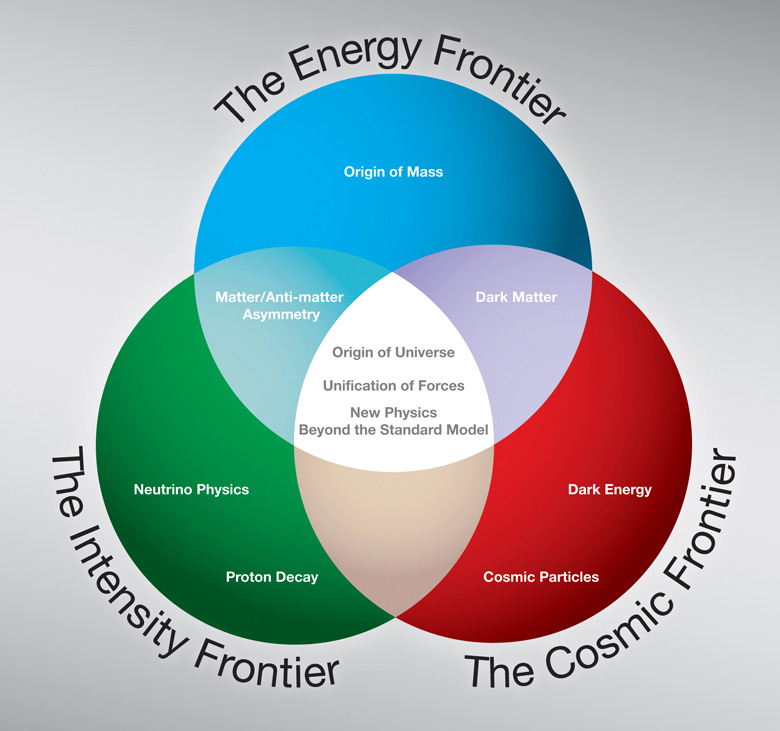
\includegraphics[scale=0.3]{three-frontiers-large}
  \caption{Fronteras de energía. Tomado de \cite{fermilab}}
  \label{fig:1}
\end{figure}

Nos encontramos ahora en una época de efervescencia experimental con
detectores de partículas instalados desde las alturas de satélites
artificiales, hasta las profundidades de laboratorios subterráneos a
kilómetros de profundidad. Esto marca una época excitante para la
física de partículas con nuevos datos experimentales disponibles en
las tres fronteras antes mencionadas. La posible correlación de datos
experimentales entre varias de las fronteras podrían permitir un
entendimiento más profundo de los constituyentes del Universo.

La \emph{Frontera de Energía} ha alcanzado la escala del Tera, la
energía a la cual se rompe la simetría electrodébil, con la puesta en
funcionamiento del Large Hadron Collider (LHC). Ubicado en un túnel a
100 metros de profundidad y con una circunferencia de 27 km, el LHC
posee cuatro detectores, dos de los cuales (ATLAS y CMS) están
especialmente diseñados para encontrar el Higgs y señales de nueva física. El LHC
ha comenzado a operar en el 2010, aunque hasta el 2012 lo hará a la
mitad de la energía para la cual fue diseñado. A partir del 2014
aproximadamente, comenzará a funcionar a la energía de diseño de
14~TeV. Para finales del 2012 el LHC habrá completado su primera fase
de operación a una energía de centro de masa de 7~TeV y habrá
acumulado al menos 8~fb$^{-1}$ de datos. Con esta luminosidad se podrá
vislumbrar una escala de energía que hasta ahora no había sido
explorada. La prioridad es la búsqueda de el bosón de Higgs del Modelo Estándar,
el cual a la fecha aún no ha sido encontrado. En el año a venir
se espera obtener la primeras evidencias de su existencia o
por el contrario fortalecer los límites de exclusión hasta un rango de masa
del orden de los 600~GeV.

En el campo de la física de partículas elementales más allá del
modelo estándar (ME), quizás el resultado experimental más importante
en los últimos años es el descubrimiento de que los neutrinos
son masivos. Dichas masas han resultado ser pequeñas aunque diferentes de
cero. Las diferencias de masa al cuadrado de los neutrinos, además de sus
correspondientes ángulos de mezcla, son necesarios para poder explicar
las observaciones de oscilaciones de neutrinos a medida que se
propagan sobre grandes distancias. Debido a que los neutrinos
interactúan sólo débilmente, los experimentos de neutrinos requieren
de detectores muy masivos y flujos muy
intensos. Los experimentos de neutrinos exploran de esta manera la
\emph{Frontera de Intensidad}. Los experimentos en esta frontera se
enfocan ahora en estudios más precisos de oscilaciones de neutrinos
así como en búsqueda de nuevas fuentes de violación de la simetría CP, mezclas de
sabores de leptones cargados, decaimientos raros, y en la
determinación de la velocidad de propagación de neutrinos altamente
energéticos. Los experimentos que utilizan flujos muy intensos a energías
inferiores que las del LHC pueden proveer información complementaria a los
posibles descubrimientos de los detectores ATLAS y CMS. Un decaimiento
raro que proviene del intercambio de una partícula de gran masa puede
contener información sobre las propiedades del estado intercambiado
aunque éste sea demasiado pesado para ser producido directamente.

Recientemente se ha venido acumulando evidencia experimental respecto
al ángulo de mezcla en el sector de neutrinos que aún falta por
determinar, mostrando que dicho ángulo no sólo es diferente de cero
sino que puede ser suficientemente grande como para permitir violación
de CP en el sector leptónico \cite{valle}. La violación de CP en el
sector leptónico es un ingrediente necesario para la generación de la asimetría
de materia-antimateria a través del mecanismo de
leptogénesis~\cite{Davidson:2008bu}.


La \emph{Frontera Cósmica} utiliza laboratorios subterráneos,
telescopios basados en tierra y telescopios instalados en satélites
para explorar la componentes oscuras de la materia y la energía, las huellas
de la inflación y el origen y destino del universo. Las observaciones
de la Frontera Cósmica han alcanzado una precisión mucho mayor de la
podría haber sido imaginada dos décadas atrás. Estos han conseguido
determinar detalles del universo primitivo los cuales son cada vez más
consistentes con el ``Modelo Estándar'' de Cosmología basado en la
constante cosmológica y en la materia oscura fría ($\Lambda$CDM), que
dan cuenta del 95\% del contenido energético del Universo. Técnicas
novedosas como lentes gravitacionales han aportado significativamente
a nuestro conocimiento del pasado cosmológico, en particular al
aumentar la evidencia experimental de que la materia oscura del
universo está compuesta de partículas masivas débilmente
interactuantes (WIMPS) \cite{Bertone:2004pz,Jungman:1995df}, formando
halos de materia oscura alrededor de las galaxias.
La materia oscura representa un gran desafío teórico y experimental,
tanto para la astrofísica moderna como para la física de partículas
\cite{Bertone:2004pz, Amsler:2008zzb, Bertone:2010,Jungman:1995df}.
Los WIMPS deben corresponder a nuevas partículas no presentes en el
ME, constituyéndose en la segunda evidencia experimental de necesidad
de física más allá del ME.  Muchos esfuerzos teóricos se han realizado
para construir teorías más allá del ME con candidatos
prometedores de materia oscura. Entre los candidatos a ser WIMPS,
tenemos la más ligera de las partículas supersimétricas, escalares
neutros adicionales, neutrinos derechos, y las partículas de
Kaluza-Klein, cada uno con diferentes implicaciones experimentales.


Las partículas que constituyen la materia oscura típicamente son
consideradas como estables, aunque también podrían ser
inestables siempre y cuando el tiempo de vida media sea mayor que la
edad del universo. Los WIMPs, si bien es cierto que interactúan débilmente
entre si, eventualmente pueden aniquilarse (o desintegrarse en el caso
de ser inestables) generando productos de aniquilación (o de decaimiento)
que contribuyen a los rayos cósmicos y que pueden llegar a los detectores
instalados en satélites artificiales orbitando la tierra. El valor de múltiples
estudios con detectores de diversos tipos de partículas y radiación
electromagnética sobre un rango muy amplio (incluyendo rayos gamma) se
hace evidente en el conocimiento detallado que se ha logrado alcanzar
y el que se espera mejorar con los experimentos que recientemente han
entrado en funcionamiento.

Cabe mencionar que el programa de detección de materia oscura se ha
centrado en la búsqueda de sus señales en los aceleradores como el LHC
\cite{Baltz:2006fm,Cho:2008tj,Nath:2010zj}, en la detección de la
energía de retroceso en la dispersión de las partículas de materia
oscura con núcleos atómicos
\cite{Green:2007rb,Bertone:2007xj,Drees:2008bv,Green:2008rd}, y la
detección indirecta a través de los estados finales de la aniquilación
y/o decaimiento de la materia oscura
\cite{Bertone:2007aw,Eichler:1989br,Arvanitaki:2008hq,Ibarra:2008jk,Ibarra:2008qg,Buckley:2009kw,Ibarra:2009tn,Ruderman:2009ta},
tales como fotones, neutrinos y la antimateria.


%%%%%%%%%%
El resultado más prometedor en esta área proviene del 2008, cuando
varios experimentos sobre rayos cósmicos como ATIC \cite{} y
los satélites PAMELA \cite{Adriani:2008zr} y Fermi
\cite{Abdo:2009zk}, comenzaron a reportar un exceso en el flujo de
electrones y positrones en rayos cósmicos.
%
Los resultados experimentales muestran un exceso
inesperado en comparación con el background convencional, tanto en el
flujo de electrones más positrones como en la fracción de positrones,
señalando la existencia de una fuente adicional de electrones y
positrones en el halo de la Vía Láctea, mientras que los datos de
antiprotones están de acuerdo con el background astrofísico esperado. 
%
Estos resultados han dado lugar a un sinnúmero de publicaciones
tratando de explicar su origen. Las medidas cada vez más precisas de
rayos gamma por parte de Fermi--LAT, pueden ayudar a discernir si el
origen de las anomalías detectadas en electrones y positrones es
debida a fuentes astrofísicas como pulsares cercanos, o a la
aniquilación o el decaimiento de materia oscura.
%
El detector de rayos cósmicos AMS-02~\cite{ams:2009}, ha sido
instalado recientemente en la estación espacial internacional para
medir el espectro y la naturaleza de los rayos cósmicos en un rango de energía
mucho más amplio y con una estadística mucho mejor que PAMELA.

Los experimentos de detección directa de materia oscura instalados en
laboratorios subterráneos como XENON100 \cite{Aprile:2011ts}
o CDMS \cite{Ahmed:2009zw,Ahmed:2010wy}, han
comenzado a explorar las regiones predichas por algunos de los modelos
más estudiados de materia oscura.
Sin embargo, hasta ahora dichos detectores no han encontrado señales
de dichas partículas. Por el contrario, existen otras medidas tomadas
con detectores tales como DAMA/LIBRA~\cite{Bernabei:2010mq},
CoGent~\cite{Aalseth:2011wp} o CRESST-II~\cite{Angloher:2011uu} que
favorecerían la existencia de partículas de materia oscura con una masa
en el rango de 6 a 15 GeV.
La situación experimental está lejos de ser sencilla, ya que por el momento
no es claro cómo conciliar los diferentes resultados de la detección directa.
No obstante, una nueva generación de detectores con masas del orden de la
tonelada como XENON1T o SuperCDMS, o con técnicas más avanzadas de
discriminación del ruido de fondo como MIMAC \cite{Billard:2011yf}
o DRIFT~\cite{Pipe:2010zz} en el caso de la detección direccional estará
próximamente disponible para así poder resolver este conflicto.
En definitiva, para los próximos años se espera una gran actividad en
el campo de la detección directa de materia oscura que permitirá
testear una porción considerable del espacio de parámetros favorecido por
la materia oscura del modelo estándar supersimétrico mínimo restringido
(cMSSM por sus siglas en inglés).\\ 
%%%%%%

Supersimetría \cite{Martin:1997ns,Haber:1984rc} es una de las teorías
propuestas para resolver el problema de la jerarquía del sector de Higgs
en el ME. El modelo estándar supersimétrico mínimo (MSSM) es, como su
nombre lo indica, la extensión supersimétrica más simple del ME.
Dicho modelo es mínimo en el sentido que contiene una mínima cantidad de campos
e interacciones.
Todas las interacciones del modelo están especificadas por las simetrías
(gauge, Lorentz, supersimetría\dots) y el superpotencial,
el cual debe ser una función holomórfica de los campos escalares del
modelo. El MSSM, además de tener la virtud de resolver el problema de jerarquía
estabilizando la masa del Higgs, unifica los acoplamientos gauge a una escala
llamada de Gran Unificación y proporciona un candidato viable para la materia
oscura. Este corresponde a la partícula supersimétrica más ligera, el
cual es estable cuando se supone la conservación de una simetría $Z_2$,
conocida también en este caso como paridad R~\cite{Ellis:1983ew} ($R_p$).
En el ME supersimétrico, además de los términos
del superpotencial que constituyen la semilla del potencial escalar y
del lagrangiano de Yukawa, las simetrías del modelo permiten los siguientes
términos:
\begin{equation}
  \label{eq:5}
  W_{\cancel{R_p}} = \mu_i\widehat{L}_i\widehat{H}_u + 
  \lambda_{i j k}\widehat{L}_i\widehat{L}_j\widehat{l}_k +
  \lambda'_{i j k}\widehat{L}_i\widehat{Q}_j\widehat{d}_k + 
  \lambda''_{ijk}\widehat{u}_i\widehat{d}_j\widehat{d}_k\,.
\end{equation}
La simetría $Z_2$, conocida en éste caso como paridad R, $R_p$,
prohíbe todos estos términos bilineales y trilineales. El modelo
resultante es conocido como modelo estándar supersimétrico con mínimo
número de operadores (MSSM). 

Además de tener la virtud de unificar a los acoplamientos gauge del
Modelo Estándar, la supersimetría a bajas energías proporciona un
candidato a materia oscura que corresponde a la partícula
supersimétrica más ligera, la cual es estable cuando se supone la
conservación de la simetría de paridad R \cite{Ellis:1983ew}. La
conservación de la simetría de paridad R prohíbe la aparición
\emph{simultánea} de operadores que violan el número bariónico y
leptónico, $\lambda'$ y $\lambda''$, evitando así el decaimiento
prematuro del protón. Otras simetrías similares a paridad R
que permiten bien sea la presencia sólo de operadores que violan número
leptónico o número bariónico también dan lugar a un protón
suficientemente estable. Estos modelos fenomenológicamente viables son
conocidos en general como modelos con violación de paridad R. Cuando
paridad R no se conserva en el Modelo Estándar supersimétrico
\cite{Barbier:2004ez}, estos operadores pueden conducir al decaimiento
de la partícula supersimétrica más ligera, teniendo profundas
implicaciones en la búsqueda de supersimetría en aceleradores y en los
experimentos de detección directa e indirecta de materia oscura. El
modelo estándar supersimétrico con rotura bilineal de paridad R
(BRpV)~\cite{}, es la versión más simple que da cuenta de las masas y
mezclas de neutrinos sin necesidad de introducir partículas
adicionales. 

Con la entrada en funcionamiento del LHC se han estado excluyendo
partes importantes de modelos supersimétricos basado en señales de
energía faltante. En general, en modelos con rotura de paridad R hay
una degradación de ésta señal haciendo más difícil su búsqueda en
colisionadores hadrónicos. En modelos con rotura de paridad R a través
de operadores que violan número bariónico, supersimetría puede quedar
incluso oculta por el background de QCD. De modo que se espera que los
modelos con rotura de paridad R ganen cada vez más importancia a
medida que se continué excluyendo el MSSM~\cite{Bomark:2011fj}.

Cuando la supersimetría se promueve a ser una simetría local de la
naturaleza, la teoría de supergravedad resultante requiere un
supermultiplete que incluya el gravitón y su supercompañero, el
gravitino~\cite{Martin:1997ns,Nilles:1983ge}. El gravitino ($\tilde
G$) adquiere masa a partir de la ruptura espontánea de la
supersimetría (llamado súper mecanismo de Higgs), la cual viene dada
por $m_{\tilde G}=\langle F\rangle/M_P$, donde $\langle F\rangle$ es el valor esperado de vacío
del campo auxiliar que rompe la supersimetría, y $M_P$ es la masa de
Planck. Por lo tanto, dependiendo del escenario de rotura de
supersimetría, el rango de la masa del gravitino va desde los eV hasta
mas allá de la escala del TeV.

La aparición natural del gravitino en supergravedad trae un problema
con el escenario de la cosmología estándar. En el Universo primitivo,
cuando el gravitino está en equilibrio térmico con el plasma, la
densidad reliquia de gravitinos es mayor que la densidad crítica, lo
que implica que el universo podría auto-contraerse. Por lo tanto, es
fundamental invocar una fase inflacionaria en el Universo con el
objetivo de diluir la densidad reliquia de gravitinos. Sin embargo,
los gravitinos también se producen en la fase de recalentamiento (a
través del decaimiento del inflatón) después de la inflación. Durante
o después de la nucleosíntesis, el decaimiento de la segunda partícula
supersimétrica más ligera o  podría
generar una lluvia electromagnética y de hadrones que echarían a
perder la predicción exitosa de las abundancias de elementos ligeros
\cite{Sarkar:1995dd}. La solución a este problema se obtiene mediante
la introducción de una violación de paridad R
\cite{Buchmuller:2007ui}, la cual permite a la segunda partícula
supersimétrica más ligera decaer en las partículas del ME
antes de la nucleosíntesis, y permite a los restantes gravitinos tener
un tiempo de vida mayor que la edad del universo. En este último caso,
el gran tiempo de vida que se requiere para un candidato de materia
oscura inestable se obtiene gracias a las débiles interacciones del
gravitino, las cuales son suprimidas por la escala de Planck y por los
pequeños acoplamientos bilineales ó trilineales que violan paridad
R. Si las masas de neutrinos son explicadas a través del mecanismo de
seesaw, el escenario con el gravitino como materia oscura y con
violación de paridad R también se ve favorecido por la teoría que
explica la asimetría entre materia y antimateria, la leptogénesis, ya
que alivia la tensión entre la alta temperatura de recalentamiento
requerida por leptogénesis y las restricciones provenientes de la
teoría de la Nucleosíntesis.  Por lo tanto, en modelos con violación de
paridad R, el gravitino como materia oscura producido en el Universo
temprano es viable y bien motivado.

Con respecto a la detección, cuando la simetría paridad R se conserva,
los gravitinos tienen interacciones muy débiles y por lo tanto ninguna
señal de la materia oscura gravitino se puede observar en los
experimentos de detección directa o indirecta. En cuanto a las señales
en los colisionadores, la producción directa de gravitinos esta muy
suprimida, pero la segunda partícula supersimétrica más ligera puede
dejar rastros en los detectores. Por otro lado, si el gravitino es
inestable (debido a la violación de paridad R) sus productos de
desintegración puede llevar a señales observables en las búsquedas
indirectas de materia oscura
\cite{Bertone:2007aw,Ibarra:2007wg,Covi:2008jy,Ibarra:2008qg}. Los
gravitinos puede ser detectados indirectamente a través del
decaimiento a rayos gamma, neutrinos o antimateria a través de los
experimentos descritos en la Frontera Cósmica. De particular interés
se tiene la región en la cual la masa del gravitino es menor que $80$
GeV, ya que el gravitino puede decaer únicamente a un neutrino y un
rayo gamma, produciendo lo que se conoce como una línea de rayos gamma
(un fotón monoenergético). Los datos del espectro de rayos gamma
extragaláctico, tomados por los satélite EGRET y FERMI, ponen fuertes
cotas sobre el espacio de parámetros de estos modelos. De hecho, en la
referencia \cite{Yuksel:2007dr} se obtuvieron restricciones sobre el
tiempo de vida del candidato a materia oscura en los modelos
supersimétricos con violación de paridad R, para un rango de masas de
$10^{-5}$ a $10$ GeV. En esta misma dirección, en la referencia
\cite{Vertongen:2011mu} se realizó una búsqueda sistemática de señales
de líneas de rayos gamma en dichos modelos, sin encontrar evidencia de
estas. Con este resultado, se obtuvieron restricciones sobre el tiempo
de vida del candidato a materia oscura para una masas entre
$1<m_{\tilde G}< 500$ GeV. Como hemos mostramos en \cite{Choi:2010jt},
y ratificado por otro grupo con datos más recientes en
\cite{Garny:2010eg}, los últimos datos de líneas de rayos gamma
publicado por FERMI-LAT excluyen la posibilidad de que las masas de
neutrinos puedan ser generadas por términos bilineales de ruptura de
paridad R si la temperatura de recalentamiento está sobre $10^9\ $GeV
como sugiere leptogénesis.  En esta región del espacio de parámetros
el gravitino es mayor de unos 10 GeV y los acoplamientos bilineales
son tan pequeños que el decaimiento de la partícula siguiente a la
LSP, la NLSP (de sus siglas en inglés), ocurre fuera del detector en
el LHC, por lo que el modelo es básicamente indistinguible del
MSSM. En éste caso los datos de detección indirecta de materia oscura
a través de rayos cósmicos serían la única forma de diferenciar el
modelo del MSSM (donde el neutralino es el candidato de materia
oscura). Sin embargo, si consideremos masas de gravitinos más
pequeñas, aunque ya no podríamos explicar bariogénesis a través de
leptogénesis, recuperamos la posibilidad de explicar las masas y
mezclas de los neutrinos a través de los operadores bilineales y
trilineales que rompen paridad R~\cite{Hirsch:2005ag}, un mecanismo,
que a diferencia del seesaw, si se puede verificar en el LHC.
En modelos supersimétricos con violación bilineal de paridad R también
la explicación de las masas y mezclas de neutrinos es especialmente
simple \cite{Hirsch:2004he,Hirsch:2008ur}: Por un lado se encuentra la
generación a nivel árbol de la escala de masa atmosférica, el ángulo
de mezcla atmosférico y el ángulo de reactor. En el otro lado, la
escala de masa solar y el ángulo de mezcla solar se obtienen por medio
de las correcciones cuánticas a un loop de la matriz de masa de los
neutrinos a nivel árbol.

La metodología desarrollada en el estudio exhaustivo de modelos
supersimétricos la hemos logrado aplicar a otros modelos de generación
radiativa de masas de neutrinos con nuevas partículas a la escala del
TeV asequibles en el LHC
\cite{Sierra:2008wj,AristizabalSierra:2006ri}.
El método para obtener una partícula estable del modelo supersimétrico
a partir de una simetría $Z_2$ como el caso de paridad R, ha sido
usado recientemente para obtener extensiones del modelo estándar que
explican materia oscura. De hecho, en el programa computacional
MicrOMEGAs~\cite{Belanger:2006is} se puede implementar cualquier
extensión del modelo estándar que posea una simetría $Z_2$ para
calcular numéricamente la densidad de reliquia de materia oscura y la
sección eficaz WIMP--nucleón, relevante para los experimentos de de
detección directa. En extensiones del modelo estándar que implementan
una simetría $Z_2$ con un singlete escalar
neutro~\cite{Yaguna:2008hd,Goudelis:2009zz,Yaguna:2011qn} o un doblete
inerte escalar~\cite{}, la partícula impar neutra y más liviana
constituye un candidato viable de materia oscura estable escalar con
implicaciones en aceleradores~\cite{} y en experimentos de detección
directa~\cite{} e indirecta~\cite{Goudelis:2009zz} de materia
oscura. En el caso de la extensión del modelo estándar con un doblete
inerte se puede tener una conexión con la frontera de intensidad si se
adicionan neutrinos derechos impares bajo la simetría $Z_2$. A
diferencia del mecanismo seesaw tradicional, en este caso
correspondiente al seesaw radiativo~\cite{}, las masas de los
neutrinos ligeros se generan al nivel de un bucle de modo que los
neutrinos derechos pueden estar en la escala del TeV con yukawas
suficientemente grandes como para ser producidos en el
LHC~\cite{Sierra:2008wj}. En general, en modelos en los cuales es
posible explicar la masa de los neutrinos total o parcialmente por
métodos radiativos, no sólo es posible dar cuenta de la pequeñez de
sus masas con respecto a la de los otros fermiones, sino también,
hacer predicciones muy concretas en aceleradores de partículas, como
el LHC.


Las observaciones astronómicas sugieren que el Universo está compuesto
en su mayor parte de materia. En el contexto del big-bang, esto
implica que en algún momento grandes cantidades de materia y
antimateria se aniquilaron dejando el pequeño exceso de materia que
constituye el Universo observable actual. El problema de explicar el
exceso inicial de materia sobre antimateria se conoce con el nombre de
bariogénesis. Dentro del modelo estándar, aunque contiene los
ingredientes necesarios, no es posible explicar bariogénesis. Los
modelos con neutrinos derechos contienen todos los ingredientes para
poder explicar bariogénesis a través de leptogénesis~\cite{}.



\subsection{Justificación:                                 }
\begin{instrucciones}
  CODI: 

  * ¿Está bien definido el problema que se quiere investigar?:
  Fenomenología de modelos más allá del ME motivados por evidencias
  fenomenológicas del ME.  
  * ¿Es clara su justificación desde el punto de vista académico,
  científico, tecnológico, social, económico y legal? (15).
  científico: contribuir a la correspondiente rama del conocimiento

  COLCI: en este ítem usted deberá describir de forma precisa y completa la
  
  * naturaleza y magnitud del problema de investigación que se quiere
  abordar:
  ** Construir modelos nuevos.
  ** Explorar modelos existentes.
  Formule claramente las preguntas concretas a las cuales se
  quiere responder en el contexto del problema planteado.
\end{instrucciones}
%Tesis
El Grupo de Fenomenología de Interacciones Fundamentales de la
Universidad de Antioquia, en colaboración con Grupos emergentes en
otras instituciones de la región conformados por egresados de
doctorado de nuestro Grupo, se ha enfocado en la investigación
científica de aspectos fenomenológicos en las tres fronteras de la
física de altas energías y la cosmología. Estas investigaciones se han
hecho en colaboración con investigadores internacionales, en
particular con científicos colombianos trabajando en el exterior que
participan en este
proyecto~\cite{Sierra:2009zq,Sierra:2008wj,AristizabalSierra:2008ye,Choi:2010jt,AristizabalSierra:2009bh};
mediante el cual buscamos dar continuidad a estos desarrollos a través
de investigaciones de impacto en la comunidad científica de éstas
áreas de frontera. En éste proyecto se continuarán explorando
diferentes extensiones del modelo estándar que explican las masas y
mezclas de neutrinos y que contienen un candidato de materia oscura
con predicciones concretas para los experimentos presentes y futuros
en las tres fronteras de la física de partículas y la cosmología.


Hemos estudiado exhaustivamente las predicciones del modelo con
ruptura bilineal de paridad R, BRpV, que incluye sólo los tres
operadores con $\mu_i$, tanto para el Tevatron como
para el LHC, asumiendo que el neutralino es la partícula
supersimétrica más liviana (LSP)
\cite{Magro:2003zb,deCampos:2005ri,deCampos:2007bn,deCampos:2008ic,deCampos:2008re,DeCampos:2010yu}. Dichas
búsquedas ya han comenzado a implementarse por las colaboración ATLAS
del LHC~\cite{:2011iu} donde se muestra el espació de parámetros
excluido en el cMSSM con BRpV hasta una luminosidad de $1\
\text{fb}^{-1}$.  En~\cite{DeCampos:2010yu} nos hemos enfocado en la
intersección entre la Frontera de Energía y la Frontera de Intensidad
al determinar el nivel de precisión con el que se puede llegar a medir
en el LHC la correlación entre decaimientos de neutralinos a muón y
tau con el ángulo de mezcla atmosférico de neutrinos: una predicción
muy concreta que de no observarse en el LHC en los próximos años
descartaría completamente el modelo como el mecanismo de generación de
masas para neutrinos. 

Cuando el gravitino es la LSP, se constituye en un candidato viable de
materia oscura inestable. Éste caso ha sido estudiado exhaustivamente
en la literatura por sus implicaciones en experimentos de rayos
cósmicos, especialmente en el caso en que . En tal caso el modelo
también explica bariogénesis a través de leptogénesis. 



También hemos explorado~\cite{} la intersección en
las tres fronteras encontrando la restricciones en el modelo BRpV
provenientes de las medidas de líneas de líneas de rayos gamma
obtenidas por Fermi--LAT cuando el gravitino es la partícula
supersimétrica más liviana y da cuenta de la materia oscura del
universo. Como los acoplamientos que violan paridad R deben ser
suficientemente grandes para explicar masas y mezclas de neutrinos,
los decaimientos que violan paridad R de la partícula supersimétrica
siguiente a la más liviana (NLSP) dominan sobre los canales de
decaimiento a gravitino, de modo que la fenomenología en aceleradores,
incluyendo las correlaciones entre las fronteras de energía e
intensidad, estudiada previamente se sigue manteniendo intacta.

Esto hace los modelos con violación de paridad R con el gravitino como
materia oscura especialmente interesantes pues genera predicciones en
la tres fronteras de las física de partículas y la cosmología, las
cuales se han venido confrontando con los resultados experimentales
muy diversos. Es así como por ejemplo se ha logrado restringir hasta
en 12 ordenes de magnitud el tiempo de vida media del gravitino, desde
los $10^{17}\ $seg (correspondientes a la edad del universo) hasta los
$10^{29}\ $seg, en el rango de masas alrededor de 10~GeV, cuando el
gravitino decae dominantemente a neutrino--fotón~\cite{}.  

\begin{gravitinodm}

  Diversos estudios han considerado las restricciones que las medidas
  de rayos cósmicos en modelos supersimétricos con violación de
  paridad R. En el caso de operadores trilineales que violan número
  leptónico se han venido reportando las restricciones sobre la masa del
  gravitino a partir de los datos de rayos cósmicos considerando sus
  decaimientos a tres cuerpos, y a un loop mediados por partículas
  gauge~\cite{}. En este proyecto extenderemos esos análisis teniendo en
  cuenta que los operadores trilineales de rotura de paridad R pueden
  inducir operadores bilineales de rotura de paridad R. En tal caso el
  gravitino tiene un nuevo canal a nivel árbol a neutrino--fotón que
  afectarán las cotas sobre la masa del gravitino especialmente en la
  región por debajo de los 80 GeV. 

  También estudiaremos las restricciones sobre la masa del gravitino
  cuando los operadores trilineales son usado para generar las masas y
  mezclas de los neutrinos, extendiendo el análisis realizado
  previamente en~\cite{}.

En el marco de los modelos supersimétricos con violación bilineal de paridad R y materia oscura de gravitinos, se supone que el gravitino es la más ligera de las partículas supersimétricas y que da cuenta de la densidad de materia oscura observada del Universo. En estos modelos, el gravitino es inestable debido a la rotura de paridad R y puede decaer en partículas del Modelo Estándar a través de las interacciones bilineales que rompen paridad R. En este escenario, todos los efectos que violan paridad R, incluyendo el decaimiento del gravitino y las masas diferentes de cero de los neutrinos, son controlados por los acoplamientos bilineales $\xi_i$. 

La detección indirecta de materia oscura involucra las búsqueda de los estados finales en las desintegraciones del gravitino, entre los que se encuentran los rayos gamma. A partir de las restricciones sobre el tiempo de vida del gravitino se pueden obtener restricciones en función de la masa del gravitino para el acoplamiento bilineal dominante $\xi_3$. Cuando se asume la unificación de las masas de los gauginos a la escala de unificación, la restricción resultante sobre $\xi_3$ es muy fuerte: $\xi_3\lesssim 10^{-7}$ para $m_{\tilde G}\gtrsim 1$ GeV.  Sin embargo, la unificación de las masas de los gauginos no es una condición que se deba asumir necesariamente en los modelos supersimétricos, lo cual implicaría que la restricción sobre $\xi_3$ puede ser relajada.

Nuestro grupo \cite{Nardi:2008ix} fue uno de los
primeros en proponer una explicación en términos de materia oscura
inestable para explicar el exceso de positrones observado por el
satélite PAMELA en el 2008 \cite{Adriani:2008zr}. Luego hemos
construido un modelo basado en supersimetría con ruptura de paridad R
a través de términos trilineales del tipo $\lambda$, caso
\ref{item:3}, para explicar la preferencia por decaimientos leptónicos
de la partícula de materia oscura, que en este caso es el
neutralino \cite{Sierra:2009zq}.
\end{gravitinodm}

\begin{bbrpvlhc}
  Existen varias extensiones del modelo BRpV que adicionan nuevas
  partículas tales como las resultantes de la adición de un
  supertriplete escalar de Higgs~\cite{}, o singletes adicionales para
  explicar el problema $\mu$. Estas extensiones se podrían
  parametrizar en términos de operadores no renormalizables que se
  podrían adicionar para tener un marco general de modelo más allá del
  BRpV. El Dr. Nicolás Bernal es un experto en extensiones más allá
  del MSSM para parametrizar el sector de Higgs~\cite{} y será de gran
  ayuda en ésta área.
\end{bbrpvlhc}

\begin{brpvlhc}
  En este proyecto pretendemos seguir explorando más correlaciones de
  de observables en el LHC con física de neutrinos para determinar con
  que nivel de precisión se podrían llegar a medir en el LHC. Cuando
  el neutralino es la LSP, los decaimientos a tres cuerpos mediados
  por sfermiones con muones y electrones en los estados finales, están
  correlaciones con el ángulo de mezcla solar, y la longitud de
  decaimiento del neutralino está correlacionada con la diferencia de
  masa atmosférica.
\end{brpvlhc}

%Frontera de energía: que esta hecho y que falta por hacer
%Hablar del modelo bilineal y su extensión como modelo efectivo

\begin{darkmatter}
  El cálculo de la densidad de neutralinos en supersimetría se conoce
  a un loop, lo cual es necesario para determinar más precisamente las
  regiones de exclusión obtenidas a partir de las medidas de detección
  directa de materia oscura. En el marco de éste proyecto,
  con la participación del estudiante de Maestría, y con el
  asesoramiento del Dr. Carlos Yaguna, se 
  calculará las contribuciones a un loop para la sección eficaz de la
  partícula escalar de materia oscura en varios  modelos con materia oscura
  escalar impar bajo una simetría $Z_2$.

  En éste proyecto se extenderá el estudio realizado
  en~\cite{Sierra:2008wj} con materia oscura tibia en el modelo seesaw
  radiativo en la intersección de las fronteras de energía e
  intensidad, para estudiar las correlaciones entre mezclas y masas de
  neutrinos con combinaciones de branchings de decaimientos de las
  partículas impares de dicho modelo en el caso de materia oscura
  fría. Para las señales más representativas realizaremos las
  simulaciones computacionales para el detector ATLAS del LHC.
\end{darkmatter}



\begin{leptogenesis}
  Aprovechando la experiencia del Dr. Diego Aristizabal en el área,
  también se explorará la posibilidad de generar leptogénesis e
  implementar simetrías no Abelianas tipo $A_4$ en el sector de Yukawa
  del seesaw radiativo para obtener ángulos de mezcla $\theta_{13}$
  suficientemente grande como sugieren las medidas experimentales
  actuales.
\end{leptogenesis}

Un modelo ideal sería uno que de cuenta de las masas y mezclas de
neutrinos, tenga un candidato a materia oscura que sirva para explicar
el exceso de positrones en experimentos de rayos cósmicos y a la vez
contenga los ingredientes para explicar bariogénesis.  En este
proyecto pretendemos formular modelos de éstas características, además
de continuar explorando otros posibles modelos que puedan dar cuenta
al menos de las dos evidencias fenomenológicas más importantes: masas
de neutrinos y materia oscura, las cuales requieren una extensión del
modelo estándar.


Con base en lo planteado anteriormente, lo que proponemos en este
proyecto es tratar de responder la siguiente pregunta: ¿Cuáles serían
las restricciones impuestas por los resultados experimentales
presentes y futuros en las tres fronteras de la física de partículas y
cosmologías sobre modelos que presenten una partícula candidata a
materia oscura y la vez generen masas para los neutrinos?
 
\subsection{Objetivos:                                     }
Implementar y complementar estudios fenomenológicos de modelos de
física más allá del Modelo Estándar, con predicciones tanto en el LHC
como en experimentos de detección
\begin{evaluador}
directa o  
\end{evaluador}
 indirecta de materia
oscura, que den cuenta de las masas de neutrinos y que posean
candidatos de materia oscura

\subsubsection{Objetivos específicos}

\begin{itemize}
\item 
  En el modelo con ruptura bilineal de paridad R con el neutralino como la LSP, determinar con
  que nivel de precisión se podría llegar a medir en el LHC la correlación entre:
%  \begin{itemize}
%  \item 
El ángulo de mezcla solar y los decaimientos a tres cuerpos mediados
    por sfermiones con muones y electrones en los estados finales.
  %\item 
La diferencia de masa atmosférica al cuadrado y la longitud de
    decaimiento del neutralino.
%  \end{itemize}

\item 
  En el modelo con ruptura bilineal de paridad R con el gravitino como
  la LSP, realizar las simulaciones de las señales del NSLP en el LHC
  en las regiones del espacio de parámetros donde el gravitino es un
  buen candidato a materia oscura y los términos bilineales pueden
  explicar los datos de oscilaciones de neutrinos.

\item 
  En el modelo con ruptura de paridad R a través de términos
  trilineales del tipo $\lambda$, extender el modelo para explicar las
  masas de neutrinos, estableciendo cual es el candidato de materia
  oscura más apropiado en ese caso.

  


\item 
\begin{darkmatter}
  En el seesaw radiativo establecer las regiones del espacio de
  parámetros donde se puede tener la densidad de reliquia de materia
  oscura y las masas y mezclas de neutrinos adecuadas. Para cada
  región establecer las señales que se esperan en el LHC y en
  experimentos de detección directa de materia oscura.  Para las
  señales más representativas, hacer simulaciones para el detector
  ATLAS del LHC.
\end{darkmatter}

\end{itemize}


\subsection{Metodología:                                   }
\begin{instrucciones}
  Esta debe reflejar la estructura lógica y el rigor científico del
  proceso de investigación, empezando por la elección de un enfoque
  metodológico específico y finalizando con la forma como se van a
  analizar, interpretar y presentar los resultados.
\end{instrucciones}
%%%

%Final
A lo largo de nuestra experiencia con el modelo con violación de
paridad R, en colaboración con otros seis investigadores de España,
Brasil y Alemanía, hemos logrado implementar todos los pasos de la
metodología usada en física de partículas para estudiar modelos de
física más allá del modelo estándar.  Ésta parte desde la formulación
misma del modelo hasta su estudio real en los aceleradores de
partículas por parte de los grupos experimentales. Esta metodología
también la hemos logrado aplicar con éxito a otros modelos. A
continuación se muestran los pasos a seguir usando como paradigma el
modelo con ruptura bilineal de paridad R y ejemplificando cada paso
con referencias concretas.
\begin{enumerate}
\item Se construye un modelo que solucione un problema fenomenológico
  del modelo estándar, como el problema de las masas de neutrinos
  \cite{Hirsch:2000ef}, o la materia oscura (o ambos
  \cite{Hirsch:2005ag}), mostrando bajo que mecanismo específico se
  soluciona el problema en cuestión. La solución del problema requiere
  introducir partículas adicionales las cuales pueden buscarse en
  detectores de partículas.
  \label{item:5}
\item Se determina el espacio de parámetros compatible con los datos
  experimentales, se calculan los branchings de decaimiento y las
  secciones eficaces y se establecen correlaciones entre estos
  observables en aceleradores con otros observables. En el caso de
  modelos con mecanismos de generación radiativa de masas de neutrinos
  las correlaciones se buscan con los datos de oscilaciones de
  neutrinos \cite{Diaz:2003as}, y en el caso de materia oscura con
  experimentos de detección directa e indirecta \cite{Choi:2010xn}.
  \label{item:6}
\item Se desarrolla un programa computacional que dado los parámetros
  de entrada del modelo entregue las secciones eficaces y los
  branching de decaimiento en un formato adecuado (el SLHA
  \cite{Allanach:2008qq}) para ser usado luego por programas de Montecarlo
  de generación de eventos como PYTHIA \cite{Sjostrand:2006za}. El
  modelo con ruptura bilineal de paridad R ha sido implementado en el
  programa computacional Spheno~\cite{Porod:2003um} (el cual tiene
  implementado el formato de salida SLHA version 2).
  \label{item:7}
\item Se divide el espacio de n-parámetros establecido en el paso
  \ref{item:6} en una malla n-dimensional. Para cada punto se corre el
  programa computacional desarrollado en el paso \ref{item:7} y los
  correspondiente datos de salida se pasan a PYTHIA usando la
  interfase SLHA. En cada punto se realiza con PYTHIA una simulación
  que consiste en generar aleatoriamente eventos de acuerdo a la
  geometría y características de detectores específicos, para
  determinar la factibilidad de descubrir las señales en aceleradores
  \cite{Magro:2003zb,deCampos:2005ri,deCampos:2007bn,deCampos:2008ic,deCampos:2008re},
  o en experimentos de detección directa o indirecta
  \cite{Choi:2010xn} de materia oscura. Este paso requiere de
  herramientas de computación de alto rendimiento en clusters de
  computadores.
  \label{item:8}
\item Como modelos muy diferentes pueden dar lugar a las mismas
  señales en detectores, se debe hacer también simulaciones en PYTHIA
  del nivel de precisión con el que se pueden determinar observables
  en aceleradores que se puedan correlacionar con observables de otros
  experimentos.
 % \begin{soloproyecto}
 %    A partir del valor experimental del ángulo de mezcla
 %  atmosférico, en el modelo con ruptura bilineal de paridad R por
 %  ejemplo, se predice que el decaimiento del neutralino a muon W, debe
 %  ser muy similar al decaimiento del neutralino a tau W. En
 %  \cite{DeCampos:2010yu} hemos determinado el nivel de precisión con
 %  el que se pude medir esta correlación en el detector ATLAS del LHC.
 %   \end{soloproyecto}
  \label{item:9}
\end{enumerate}
Las simulaciones se realizan con el fin de desarrollar todas las
herramientas necesarias para que los grupos experimentales de los
aceleradores puedan comparar los datos obtenidos con modelos
específicos y puedan descubrir o poner cotas sobre las nuevas
partículas propuestas. En el caso de detección directa o indirecta de
materia oscura donde las señales están preestablecidas, la
simulaciones se realizan para poder comparar con los datos obtenidos o
que se pueden llegar a obtener. En el caso del modelo con ruptura
bilineal de paridad R, ya se han hecho búsquedas en
Tevatron~\cite{Brigliadori:2008vf} y se están implementando búsquedas
con datos reales en el LHC en grupos de trabajo de ATLAS y
LHCb. Además se han establecido la posibles señales que se pueden
observar en experimentos de detección indirecta de materia oscura a
través de rayos cósmicos \cite{Choi:2010jt}.

\begin{proyecto}
  En el marco de este proyecto se simularán dos correlaciones
  adicionales que existen en el modelo con ruptura bilineal de paridad R:
  Cuando el neutralino es la LSP, los decaimientos a tres cuerpos
  mediados por sfermiones con muones y electrones en los estados
  finales, están correlaciones con el ángulo de mezcla solar, y la
  longitud de decaimiento del neutralino está correlacionada con la
  diferencia de masa atmosférica.
\end{proyecto}

\begin{proyecto}
  En el modelo donde la ruptura bilineal de paridad R puede explicar
  tanto las masas de neutrinos como la densidad de reliquia de materia
  oscura cuando la LSP es el gravitino se realizaran los pasos
  \ref{item:7} y \ref{item:8} de la metodología.
\end{proyecto}

\begin{evaluador}
  \begin{darkmatter}
  \begin{proyecto}
  Para el seesaw radiativo, en la literatura básicamente sólo se ha
  realizado el paso \ref{item:5}, aunque para algunas regiones del
  espacio de parámetros donde la partícula más liviana de paridad
  impar (LOP de sus siglas en inglés) es escalar se ha llegado hasta
  el paso \ref{item:8}~\cite{Bergman:2007pm}. En este proyecto haremos un
  estudio sistemático del modelo incluyendo todos los pasos de la
  metodología. Cómo el modelo está basado en una simetría $Z_2$,
  implementaremos el modelo en MicrOMEGAS~\cite{Belanger:2010gh} donde
  además de calcular la densidad de reliquia, y la sección eficaz
  WIMP-nucleon, se pueden obtener todas las secciones eficaces y
  amplitudes de decaimiento con el formato SLHA, lo que facilitará las
  simulaciones para el LHC.
\end{proyecto}
\end{darkmatter}
\end{evaluador}

\begin{proyecto}
  Para el modelo con con ruptura de paridad R a través de términos
  trilineales del tipo $\lambda$, sólo hemos realizado el paso
  \ref{item:5}, como un modelo que contiene un candidato inestable de
  materia oscura que explica el exceso de positrones observado por
  PAMELA. En este proyecto queremos adicionar al modelo la posibilidad
  de explicar las masas y mezclas de neutrinos y avanzar en los demás
  pasos de la metodología.
\end{proyecto}

A través de todo el proyecto se requiere de una infraestructura de
computación de alto rendimiento adecuada, que garantice una
disponibilidad permanente de poder de computo para las diferentes
simulaciones y programas computacionales que requiere el proyecto. El
grupo ha venido consolidando sus herramientas de computación con la
adquisición de un servidor Blade con capacidad para 8 nodos, aunque de
momento sólo tiene un nodo instalado. Toda esta experiencia le ha
permitido consolidar un grupo de desarrolladores y administradores de
software científico que ahora conforman La división de ciencias de la
computación del grupo la cual es ahora la encargada de administrar el
Centro Regional de Simulación y Cálculo Avanzado (CRESCA) y ofrece
servicio de computación científica.  Una de las metas prioritarias es
la unificar el poder de computo de los Grupos de Investigación de la
Universidad, como el servidor Blade del grupo, en un Grid
Institucional que la vez éste conectado con Grid-Colombia. En el
proyecto solicitamos la renovación del contrato al Administrador de
Sistemas, que dedicaría parte de su tiempo para la administración de
CRESCA y la implementación del Grid Institucional de computación de
alto rendimiento.
\begin{ideas}
  

Para un modelo que incluya mecanismos de generación radiativa de masas de neutrinos se determina el espacio de parámetros compatible con los datos experimentales sobre física de neutrinos, se calculan los branchings de decaimiento y las secciones eficaces y se establecen correlaciones entre estos observables y los datos de física de neutrinos [7]. Para el caso de VBPR todo esto ya ha sido implementado en el programa computacional SPheno [8]. Finalmente se hace una simulación con PYTHIA [9] de la factibilidad de descubrir el modelo en aceleradores, como hemos venido haciendo con VBPR en [1], y de la viabilidad de medir las correlaciones establecidas, que es uno de los objetivos del proyecto.

Como hemos ya hecho en [3], obtendremos resultados numéricos para los flujos de rayos cósmicos  producidos en el decaimiento del CMOI usando PYTHIA. A partir de los resultados se analizará el tiempo de vida del CMOI  en términos de su masa con el fin de obtener y analizar cuáles serían las regiones del espacio de parámetros restringidas o excluidas por los experimentos de rayos cósmicos.

En este proyecto haremos una implementación del modelo de seesaw radiativo en Micromegas  con el cual se pueden hacer los cálculos de densidad de reliquia, secciones eficaces, amplitudes de decaimiento, etc. Una vez establecidas las regiones del espacio de parámetros relevantes, se procederá con el método para mecanismos de generación radiativa de masas de neutrinos descrito anteriormente.
\subsection{Actividades:                                   }

\subsection{Resultados esperados:                          }
\begin{instrucciones}
CODI:  Impacto y relevancia:
¿El proyecto permite la generación de conocimiento científico o aporta a la resolución de problemas concretos de la realidad? ¿Son suficientes y adecuados los mecanismos de comunicación y socialización de resultados? 

 COLCI: Formule los resultados directos verificables que se
alcanzarán con el desarrollo de los objetivos específicos del proyecto. Estos deben ser coherentes
con los objetivos y con la metodología planteada.



  \begin{enumerate}
  \item \textbf{Relacionados con la generación de conocimiento y/o nuevos desarrollos
 tecnológicos:} Incluye resultados/productos que corresponden a nuevo
 conocimiento científico o tecnológico o a nuevos desarrollos o adaptaciones de
 tecnología que puedan verificarse a través de publicaciones científicas,
 productos o procesos tecnológicos, patentes, normas, mapas, bases de datos,
 colecciones de referencia, secuencias de macromoléculas en bases de datos de
 referencia, registros de nuevas variedades vegetales, etc.
\item \textbf{Conducentes al fortalecimiento de la capacidad científica
  nacional:} Incluye resultados/productos tales como formación de
  recurso humano a nivel profesional o de posgrado (trabajos de grado
  o tesis de maestría o doctorado sustentadas y aprobadas),
  realización de cursos relacionados con las temáticas de los
  proyectos (deberá anexarse documentación soporte que certifique su
  realización), formación y consolidación de redes de investigación
  (anexar documentación de soporte y verificación) y la construcción
  de cooperación científica internacional (anexar documentación de
  soporte y verificación).
\item \textbf{Dirigidos a la apropiación social del conocimiento:}
  Incluye aquellos resultados/productos que son estrategias o medios
  para divulgar o transferir el conocimiento o tecnologías generadas
  en el proyecto a los beneficiarios potenciales y a la sociedad en
  general. Incluye tanto las acciones conjuntas entre investigadores y
  beneficiarios como artículos o libros divulgativos, cartillas,
  videos, programas de radio, presentación de ponencias en eventos,
  entre otros.
  \end{enumerate}

  Para cada uno de los resultados/productos esperados identifique (en
  los cuadros a continuación) indicadores de verificación (ej:
  publicaciones, patentes, registros, videos, certificaciones, etc.)
  as\'\i{} como las instituciones, gremios y comunidades beneficiarias,
  nacionales o internacionales, que podrán utilizar los resultados de
  la investigación para el desarrollo de sus objetivos, políticas,
  planes o programas:

\end{instrucciones}

\begin{instrucciones}
  Los impactos no necesariamente se logran al finalizar el proyecto, ni
con la sola consecución de los resultados/productos. Los impactos
esperados son una descripción de la posible incidencia del uso de los
resultados del proyecto en función de la solución de los asuntos o
problemas estratégicos, nacionales o globales, abordados. Generalmente
se logran en el mediano y largo plazo, como resultado de la aplicación
de los conocimientos o tecnologías generadas a través del desarrollo
de una o varias líneas de investigación en las cuales se inscribe el
proyecto. Los impactos pueden agruparse, entre otras, en las
siguientes categorías: sociales, económicos, ambientales, de
productividad y competitividad. Para cada uno de los impactos
esperados se deben identificar indicadores cualitativos o
cuantitativos verificables as\'\i:
\end{instrucciones}


Nos encontramos en una época única en la que se esperan grandes
descubrimientos en el área de física de altas energías.
\begin{soloproyecto}
El LHC ha
comenzado a explorar la escala del TEV desde el 2010. Hasta el 2012
estará acumulando datos a 7\,TeV de energía de centro de masa, y a
partir del 2014 comenzará a funcionar a su energía de diseño de 14
TeV. El satélite Planck fue lanzado en el 2009 y se espera que
entregue datos definitivos sobre los parámetros astronómicos en el
2012. La misión complementará y mejorará las observaciones hechas por
el WMAP. Éste año, XENON100 ha entregado sus primeros datos que
comienzan a restringir las regiones del espacio de parámetros de
algunos modelos de materia oscura, y para el 2015 se espera que los
datos de XENON1T cubran completamente la región de materia oscura
predicha por el MSSM restringido. AMS-02 es un detector de rayos
cósmicos que será llevado a la estación espacial internacional a bordo
de la última misión del transbordador Endeavor el 29 de abril de
2011. Se espera que compruebe y mejore las medidas de PAMELA sobre
exceso en el flujo de positrones de rayos cósmicos.  
\end{soloproyecto}
 Hemos entrado en
una nueva era de la física que, de obtener los resultados esperados,
combinaría los descubrimientos de nuevas partículas, a los cada vez
mejor establecidos resultados de física de neutrinos y observaciones
cosmológicas sobre materia oscura. El resultado de este proyecto es
aportar a esta área de la ciencia con nuevas propuestas de señales
para ser buscadas en estos detectores (subterráneos y en el espacio) y
con la interpretación de los resultados que surjan de ellos en
términos de los modelos propuestos, en los cuales se añaden partículas
nuevas al modelo estándar de la partículas elementales. Estos
resultados se reflejarán en la publicación de al menos dos artículos
científicos en el área con la participación de un estudiante de
Doctorado, y en la presentación de los resultados en al menos una
conferencia internacional. Además de dar pie a la formulación de
nuevos proyectos de investigación para ser presentado en convocatorias
externas.


De especial importancia es el nuevo paradigma científico que surgirá
de la combinación de todos esos resultados experimentales. Por ejemplo
el descubrimiento en el LHC de la partícula escalar elemental predicha
por el Modelo Estándar, el Higgs, establecería finalmente las teorías
gauge con rompimiento espontáneo de simetría como el principio
fundamental para describir las interacciones subatómicas, redondeando
décadas de desarrollo científico.  El estudio detallado de las
propiedades del Higgs, acompañado posiblemente de señales
de nueva física, podría marcar el camino para encontrar el mecanismo
de generación de masas y mezclas de neutrinos, así como la
determinación de la partícula que compone la materia oscura del
Universo. A más tardar al finalizar ésta década, se espera tener
respuesta a todos estos interrogantes. Todo esto tendrá un impacto en la
enseñanza de la física a todos los niveles. Además el descubrimiento
del Higgs, que sería la primera partícula escalar elemental, daría un
mejor fundamento teórico a los modelos inflacionarios en cosmología y
a la interpretación de la energía oscura como la causante de la
expansión acelerada del Universo. El otro escenario posible en el que
no se encuentre al Higgs del modelo estándar, debe dar lugar a datos
experimentales suficientes para dilucidar cual es realmente el
mecanismo de ruptura de la simetría electrodébil. Nuestro grupo es el
más directamente llamado a difundir estos avances en nuestro entorno social,
como lo ha venido haciendo a través de conferencias y cursos de
extensión en los últimos años. Es importante que nuestro país siga
participando en el desarrollo de la física fundamental, no sólo con la
participación de grupos teóricos como el nuestro, sino también con
grupos experimentales de física de altas energías como lo viene
haciendo en las colaboraciones ATLAS y CMS del LHC con grupos de la
Universidad Antonio Nariño y de los Andes respectivamente. Con ellos,
y con los otros grupos teóricos del país, hemos venido colaborando y
organizando congresos en el área en los últimos años para consolidar
ésta área de investigación en el país.

El principal aporte de un Grupo como el nuestro al desarrollo del país
es la formación de talento humano con capacidad de hacer investigación
científica al más alto nivel. Para ello es prioritario que nuestro
Grupo siga produciendo productos de gran impacto en la comunidad
mundial de física de altas energías con participación de nuestros
estudiantes de pregrado y posgrado.  Aunque de momento los doctores
que formamos son rápidamente reabsorbidos en el ámbito académico,
esperamos que a futuro, como pasa en otros países donde profesionales
de este tipo son muy apreciados en empresas de innovación tecnológica,
los nuestros puedan llegar a hacer aportes significativos a otros
sectores de la sociedad. También hemos logrado capacitar nuestro
equipo técnico en herramientas de computación científica y de
administración de redes en Linux.


De ser aprobado, éste proyecto nos permitiría participar en esta
excitante era del desarrollo científico que coincide con
los primeros años de funcionamiento del LHC.  Se espera que entre los
resultados de los próximos años LHC, no solo esté el del
descubrimiento del Higgs, sino también de alguna señal de física más
allá del modelo estándar que explique los problemas fenomenológicos y
teóricos del Modelo Estándar. En los próximos años también se espera
que los experimentos de detección directa, o indirecta a través de
rayos cósmicos, entreguen una evidencia definitiva de materia oscura.



\subsection{Cronograma:                                    }

\subsection{Equipo de trabajo:}
\begin{tabular}{|l|l|l|l|}\hline
Recurso humano (rol)& Responsabilidad& Unidades (días, meses)& \# de unidades\\\hline
&&&\\\hline
\end{tabular}

\subsection{Presupuesto}
\begin{instrucciones}
  Por favor siga el modelo de la tabla que encontrará en este punto para la presentación del presupuesto.
\end{instrucciones}
\begin{tabular}{|l|l|l|l|}\hline
  \multirow{2}{*}{Rubros}&\multicolumn{2}{c}{Fuentes}\vline&\multirow{2}{*}{Total}\\
  \cline{2-3} & Colciencias & Contrapartida & \\\hline 
 & & &\\\hline
 & & &\\\hline
 & & &\\\hline
 & & &\\\hline
TOTAL (en pesos) & & &\\\hline
Total en porcentaje & & &\\\hline
\end{tabular}

\subsection{Plan de acción.}
\begin{tabular}{|l|l|l|l|l|l|}\hline
  \multirow{2}{*}{Objetivo} & \multirow{2}{*}{Estrategia} & \multirow{2}{*}{Indicador}  & \multicolumn{3}{|c|}{Metas}\\
\cline{4-6} 
& & & Bimestre 1 &Bimestre 2 & Bimestre 3\\\hline 
&&&&&\\\hline
\end{tabular}



%%% Local Variables: 
%%% mode: latex
%%% TeX-master: "proyecto"
%%% End: 
